\documentclass[UTF8,11pt,a4paper]{ctexart}

\usepackage[a4paper,margin=2.2cm]{geometry}
\usepackage{booktabs}
\usepackage{longtable}
\usepackage{array}
\usepackage{tabularx}
\usepackage{multirow}
\usepackage{enumitem}
\usepackage{xcolor}
\usepackage{hyperref}
\usepackage{fancyhdr}
\usepackage{titlesec}
\usepackage{setspace}
\usepackage{graphicx}
\usepackage{amsmath}
\usepackage{amssymb}
\usepackage{url}
\usepackage{float}
\usepackage{fancyvrb}

\hypersetup{
  colorlinks=true,
  linkcolor=blue!50!black,
  urlcolor=blue!50!black,
  pdftitle={outerCube：低精度矩阵乘中的局部归约深度、累加器压力与微架构边界},
  pdfauthor={},
  pdfsubject={Circuit-level analysis of low-precision matrix multiplication},
  pdfkeywords={outer product, inner product, FP8, matrix multiplication, accumulator, microarchitecture}
}

\setmainfont{Times New Roman}
\setsansfont{Helvetica Neue}
\setmonofont{Menlo}
\setCJKmainfont{PingFang SC}
\setCJKsansfont{PingFang SC}
\setCJKmonofont{STHeiti}

\pagestyle{fancy}
\fancyhf{}
\lhead{outerCube 微架构分析}
\rhead{\thepage}
\setlength{\headheight}{14pt}

\setlist[itemize]{leftmargin=2em}
\setlist[enumerate]{leftmargin=2.4em}
\setstretch{1.18}
\DefineVerbatimEnvironment{code}{Verbatim}{fontsize=\small}

\titleformat{\section}{\Large\bfseries}{\thesection}{0.8em}{}
\titleformat{\subsection}{\large\bfseries}{\thesubsection}{0.8em}{}
\titleformat{\subsubsection}{\normalsize\bfseries}{\thesubsubsection}{0.8em}{}

\newcommand{\ku}{\ensuremath{k_u}}
\newcommand{\modea}{Mode A}
\newcommand{\modeb}{Mode B}
\newcommand{\outercube}{\textit{outerCube}}

\title{\textbf{\outercube{}：低精度矩阵乘中的局部归约深度、累加器压力与微架构边界}}
\author{}
\date{}

\begin{document}

\maketitle

\begin{abstract}
\outercube{} 提出了一种面向低精度矩阵乘的双模式矩阵单元。该设计以 8 个 bank
组织 tile 级 outer-product accumulation engine，并统一使用 FP32 accumulator
承接 FP16/BF16/FP8/MXFP4/HiFP4 的计算结果。其目标是在大 K dense GEMM 中维持
高复用与高吞吐，同时在小 K 场景下降低 K-ceiling 浪费。然而，对低精度矩阵乘而言，
真正决定电路代价和数值稳健性的往往不是“外积”或“内积”的标签，而是局部归约深度、
high-precision psum 更新频率以及 partial sum 的组织方式。

本文基于公开规格、相关文献和可推导的局部归约模型，对 \outercube{} 进行电路级分析。
本文引入局部归约粒度 \ku{}，用于刻画单个输出元素在一次 high-precision psum 更新之前
已经融合的乘积项个数，并据此重构 \modea{} 与 \modeb{} 的真实微结构。分析表明，
\modea{} 并非 naive outer-product update，而是块外积数据流与局部小点积归约的折中；
相反，\modeb{} 在 FP16/BF16 和 FP8 下分别退化为 $\ku=1$ 和 $\ku=2$ 的小粒度外积更新，
使 FP32 psum 更新频率、TRegFile 读流量和 drain 压力显著上升。

本文进一步指出，\outercube{} 的 reduced-precision adder tree 虽然抓住了局部归约
代价这一关键问题，但“zero-padding 后无精度损失”的表述缺乏充分的浮点依据，因为
mantissa 位宽、exponent alignment、guard/sticky bit 以及舍入顺序会共同决定最终误差。
综合来看，\outercube{} 的主要价值在于 \modea{} 所体现的 block outer-product 组织，
而其主要风险则集中于 \modeb{} 过低的局部归约深度和统一 FP32 psum 带来的高频更新开销。
基于这些分析，本文给出一个面向架构决策的结论：当目标是大 K、dense GEMM 的吞吐与数据复用时，
优先考虑 block outer-product dataflow，但必须同时配备足够的局部归约深度；当目标是更直接的
局部 K 归约语义、较强的数值可控性或较小 K 工作负载时，inner-product primitive 更自然。
对 FP16/BF16/FP8 而言，真正应避免的并不是“外积”本身，而是 \ku{} 过小、使高精度 accumulator
在 product 级反复介入的纯串行外积累加。
\end{abstract}

\section{引言}

低精度矩阵乘单元常被粗略地分为 ``外积'' 与 ``内积'' 两派，但这种二分在真实硬件中往往
过于粗糙。现代矩阵单元既要处理 dense GEMM 的高吞吐与高复用，又要处理 FP8、FP4
甚至更低精度下的累加误差、overflow、underflow 与 psum 带宽压力。于是，许多设计
在全局数据流上偏外积，在局部归约上偏小内积，在 ISA 层暴露 tile MMA，在微架构层
隐藏多级缓冲和 reduction tree。这种多层混合导致简单的 ``外积好'' 或 ``内积好'' 都不再
成立。

\outercube{} 是一个很有代表性的例子。其文档明确宣称自身是
``large-scale outer-product accumulation engine''，并提出两个执行模式：
\modea{} 让 8 个 bank 沿 K 并行后进入共享 adder tree；
\modeb{} 让 8 个 bank 各自处理不同 M-block，绕开 inter-bank reduction 并保留
独立 accumulator。表面看，这是一种兼顾大 K 与小 K 工作负载的灵活设计；但从电路
角度看，两个模式的局部归约深度完全不同，导致它们的数值与面积权衡也完全不同。

本文把问题收敛到最底层电路。我们不讨论软件 blocking，也不讨论 ISA 层 ``矩阵乘是否
写成 outer product'' 的表面语义，而是讨论：每一个输出元素在进入高精度 psum 之前，
到底已经吸收了多少乘积项；这决定了 high-precision accumulation 被触发的频率，也决定
了设计更接近 outer-product update 还是更接近 local dot-product reduction。

本文的贡献如下：

\begin{itemize}
  \item 给出一个统一的局部归约粒度指标 $\ku$，用它重新解释 \outercube{} 的
  \modea{} 与 \modeb{}。
  \item 说明 \modea{} 为何在 dense GEMM 上是合理的 block outer-product compromise。
  \item 说明 \modeb{} 为什么在 FP16/FP8 下退化为小 $\ku$ 外积，从而在电路上更贵。
  \item 论证 reduced-precision tree ``无精度损失'' 的说法为何过强。
  \item 给出面向架构决策的选择框架，说明何时应优先选择 inner-product primitive，
  何时应优先选择 outer-product dataflow，以及何时应采用混合方案。
\end{itemize}

\section{背景与评审视角}

\subsection{矩阵乘的两种视角}

矩阵乘 $C = A \times B$ 可写为两种等价形式：

\begin{align}
  C_{ij} &= \sum_k A_{ik} B_{kj} \\
  C &\mathrel{+}= A_{:,k} B_{k,:}
\end{align}

前者是内积视角，后者是外积视角。若只从数学角度看，两者没有本质差异；但从硬件角度看，
二者牵动的代价完全不同：

\begin{itemize}
  \item 内积强调沿 K 维做归约，因此更自然地暴露为 dot product 或 small SoP unit。
  \item 外积强调一次广播一组输入并更新一片输出，因此更自然地暴露为 rank-1 或 rank-k
  update，以及 systolic / block-outer-product dataflow。
\end{itemize}

真正决定代价的不是数学写法，而是 \textbf{partial sums 在何处、以何种精度、以何种频率被更新}。

\subsection{一个直观例子：同一件事，既可以看成内积，也可以看成外积}

为了让后文的讨论更直观，这里用一个最简单的 $2\times 2$ 例子说明两种视角。

设
\begin{equation}
  A=
  \begin{bmatrix}
    a_{11} & a_{12}\\
    a_{21} & a_{22}
  \end{bmatrix},
  \qquad
  B=
  \begin{bmatrix}
    b_{11} & b_{12}\\
    b_{21} & b_{22}
  \end{bmatrix}
\end{equation}

则结果矩阵 $C=A\times B$ 为
\begin{equation}
  C=
  \begin{bmatrix}
    a_{11}b_{11}+a_{12}b_{21} & a_{11}b_{12}+a_{12}b_{22}\\
    a_{21}b_{11}+a_{22}b_{21} & a_{21}b_{12}+a_{22}b_{22}
  \end{bmatrix}
\end{equation}

从内积视角看，$C$ 的每个元素都是一行乘一列。例如，
$C_{11}= [a_{11},a_{12}] \cdot [b_{11},b_{21}]$，
$C_{12}= [a_{11},a_{12}] \cdot [b_{12},b_{22}]$。这种写法最符合线性代数课本里的直觉：
每个输出元素各算各的，只是都要沿着同一个 $K$ 维把乘积加起来。

从外积视角看，可以把 $A$ 的第 1 列与 $B$ 的第 1 行拿出来，先生成一个 rank-1 更新：
\begin{equation}
  \begin{bmatrix}
    a_{11}\\
    a_{21}
  \end{bmatrix}
  \begin{bmatrix}
    b_{11} & b_{12}
  \end{bmatrix}
  =
  \begin{bmatrix}
    a_{11}b_{11} & a_{11}b_{12}\\
    a_{21}b_{11} & a_{21}b_{12}
  \end{bmatrix}
\end{equation}

再把 $A$ 的第 2 列与 $B$ 的第 2 行做一次同样的更新：
\begin{equation}
  \begin{bmatrix}
    a_{12}\\
    a_{22}
  \end{bmatrix}
  \begin{bmatrix}
    b_{21} & b_{22}
  \end{bmatrix}
  =
  \begin{bmatrix}
    a_{12}b_{21} & a_{12}b_{22}\\
    a_{22}b_{21} & a_{22}b_{22}
  \end{bmatrix}
\end{equation}

把这两个小矩阵相加，得到的就是同一个 $C$。因此，“内积”和“外积”首先是
\textbf{看待同一矩阵乘过程的两种方式}。前者更强调“一个输出元素怎么得到”，后者更强调
“一次送入一组输入后，可以同时更新多少个输出元素”。

\begin{figure}[H]
  \centering
  \begin{minipage}[t]{0.48\textwidth}
    \centering
    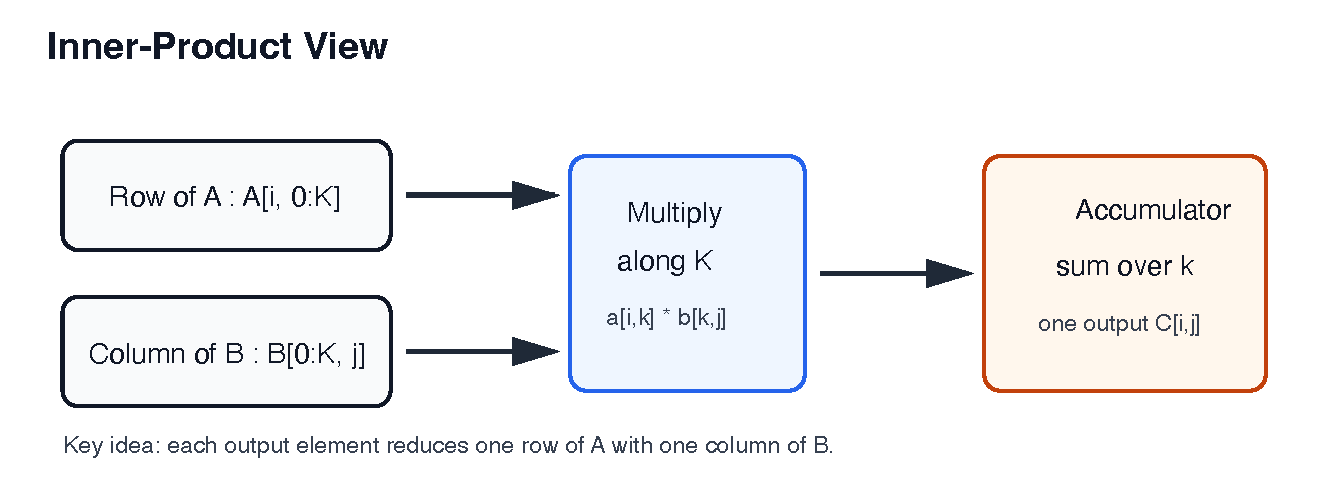
\includegraphics[width=\textwidth]{figures/inner-product-dataflow.pdf}
  \end{minipage}
  \hfill
  \begin{minipage}[t]{0.48\textwidth}
    \centering
    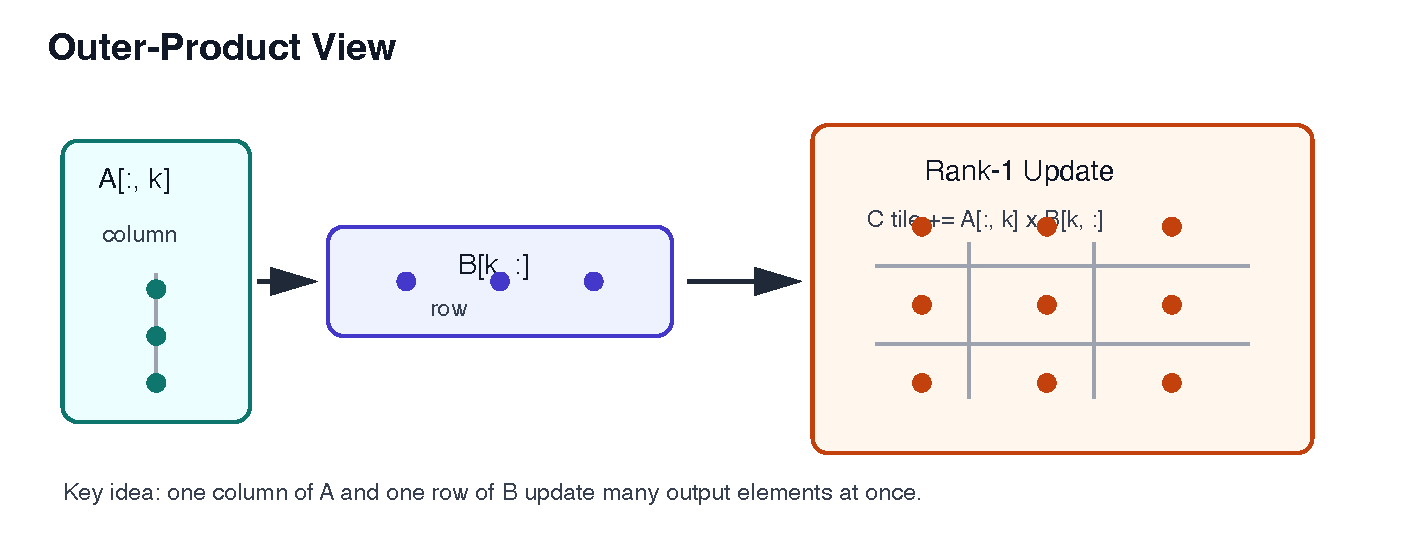
\includegraphics[width=\textwidth]{figures/outer-product-dataflow.pdf}
  \end{minipage}
  \caption{内积式与外积式矩阵乘的数据流示意。左图强调“一个输出元素如何沿 K 维完成归约”，右图强调“一个输入对如何同时更新一片输出 tile”。}
  \label{fig:inner-outer}
\end{figure}

\subsection{伪代码：内积、外积与 tile MMA}

为了让术语和后文的硬件讨论对应起来，这里给出三类常见写法的伪代码。它们在数学上等价，
但对数据复用和 psum 更新位置的暗示完全不同。

\noindent\textbf{Algorithm 1.} Inner-product GEMM
\begin{code}
for i in 0 .. M-1:
  for j in 0 .. N-1:
    acc = 0
    for k in 0 .. K-1:
      acc += A[i, k] * B[k, j]
    C[i, j] = acc
\end{code}

\noindent\textbf{Algorithm 2.} Outer-product GEMM
\begin{code}
initialize C to zero
for k in 0 .. K-1:
  a_col = A[:, k]
  b_row = B[k, :]
  for i in 0 .. M-1:
    for j in 0 .. N-1:
      C[i, j] += a_col[i] * b_row[j]
\end{code}

\noindent\textbf{Algorithm 3.} Tile MMA
\begin{code}
for each output tile (tm, tn):
  load C_tile
  for tk in K tiles:
    A_tile = load A[tm, tk]
    B_tile = load B[tk, tn]
    C_tile = MMA(A_tile, B_tile, C_tile)
  store C_tile
\end{code}

\subsection{为什么硬件特别关心 K 维、partial sum 和 accumulator}

普通读者最容易困惑的地方在于：既然内积和外积在数学上等价，为什么硬件圈会如此在意它们的差别？
原因在于，芯片不是只关心算对，还关心 \textbf{数据怎么搬、加法在哪里做、以及中间结果要保存多久}。

在矩阵乘里，$K$ 维是归约维。无论采用内积还是外积，最终都必须把多个乘积项加到同一个输出元素上。
这些还没加完的中间结果，本文统一称为 \textbf{partial sum}，简称 \textbf{psum}。负责保存和更新
psum 的寄存器或缓冲，可以统称为 \textbf{accumulator}。如果把矩阵乘想象成记账，那么乘法只是不断
生成“新账单”，而 accumulator 才是那个不断把账单并入总账的地方。

这也是为什么硬件讨论中经常出现 tile、bank 和 accumulator 这些词。所谓 tile，就是一次送入
硬件处理的一小块矩阵；bank 可以理解为并行工作的若干子阵列；accumulator 则是这些子阵列最终要把
中间结果写回去的“总账本”。一个设计真正昂贵的地方，很多时候不是乘法器数量，而是：

\begin{itemize}
  \item 同一份输入能被多少个乘法器复用；
  \item psum 需要被读取、更新和写回多少次；
  \item 每次更新 psum 时，是否都要动用较宽、较慢、较耗能的高精度加法路径。
\end{itemize}

\subsection{为什么低精度不等于累加一定便宜}

另一个常见误解是：既然输入已经降到 FP8、INT8 甚至 FP4，那么矩阵乘一定会变得很便宜。
这对乘法器通常是成立的，但对累加器不一定成立。

原因很简单。即使单次乘法已经很低精度，多个乘积项相加后，数值范围仍然会迅速增长。以定点数为例，
若每个乘积都可能达到某个最大值，那么把 $K$ 个这样的乘积加起来，累加器大致还要再多出
$\log_2 K$ 位才能避免溢出。对浮点数来说，问题更复杂：不仅要处理 mantissa 的相加，还要处理
exponent alignment、normalization 和 rounding。于是就会出现一种现象：
\textbf{乘法器已经变便宜了，但负责更新 psum 的高精度路径依然很贵。}

因此，低精度矩阵乘真正的关键问题常常不是“能不能做很多低精度乘法”，而是“能否减少高精度 psum
更新的频率”。这正是本文引入局部归约粒度 \ku{} 的原因。它并不是一个抽象数学记号，而是在衡量：
一个设计到底是每来一个乘积就更新一次总账，还是先在局部凑成若干小和，再去更新总账。

\subsection{顺序外积累加会放大指数对齐误差}

这里需要进一步区分两件容易混淆的事情：\textbf{外积数据流} 与 \textbf{纯外积串行累加} 并不是同一概念。
前者描述的是输入和输出 tile 的复用方式；后者描述的是最小数值更新单元。如果最小更新单元是
\begin{equation}
  \hat{c}_{t+1} = fl(\hat{c}_t + p_t), \qquad p_t = a_t b_t,
\end{equation}
那么这个过程本质上就是浮点数值分析里的 recursive summation。此时，当前累计值 $\hat{c}_t$ 的指数
会在每一步都参与 exponent alignment，新的乘积 $p_t$ 需要不断按照 $\hat{c}_t$ 的量级右移、规格化并舍入。
一旦 $\hat{c}_t$ 已经足够大，而 $p_t$ 相对较小，就会出现经典的 swamping 现象：$p_t$ 的低位在对齐时被移出，
从而对最终结果几乎不再产生贡献。

这一点可以用标准误差分析表述得很清楚。Higham 对 floating-point summation 的分析指出，通常的
recursive summation 满足
\begin{equation}
  |\hat{s}-s| \le \gamma_{K-1}\sum_{t=0}^{K}|x_t|,
  \qquad
  \gamma_n = \frac{nu}{1-nu},
\end{equation}
其最坏情形误差常数与 $K$ 近似成正比 \cite{higham}. 更重要的是，Higham 还指出一阶误差实际上是
\textbf{由各步 partial sum 加权的舍入误差之和}；也就是说，越到后面的累加，其误差越受到当前累计值大小的影响
\cite{higham}. 把这一结论翻译到纯外积串行累加上，就是：当 $c$ 在每一步都进入加法器时，$c$ 的指数会反复支配
新乘积的对齐位置，因此误差并不是“只由输入精度决定”，而是会随着累加深度持续放大。

相反，如果把乘积先按小组归约，例如
\begin{equation}
  g_0 = fl(p_0 + p_1 + p_2 + p_3), \qquad
  g_1 = fl(p_4 + p_5 + p_6 + p_7),
\end{equation}
再执行 $\hat{c}\leftarrow fl(\hat{c}+g_0)$、$\hat{c}\leftarrow fl(\hat{c}+g_1)$，那么 $c$ 的指数只会在
每个 group 的最后一次累加中起作用，而不是在每个乘积上都起作用。这种做法在数值上更接近 pairwise 或 grouped
summation。Higham 的分析表明，pairwise summation 的误差常数是 $\log_2 n$ 量级而不是 $n$ 量级
\cite{higham}. 虽然硬件中的 group reduction 未必严格等价于一棵完美平衡树，但其核心收益是一致的：
\textbf{把高精度 accumulator 对局部乘积的“逐项支配”改成“按组支配”。}

这也解释了为什么 fused dot-product 单元值得付出额外电路代价。Lutz 等人的 FP8-DOT4 工作明确指出，
所谓 fused 的关键并不只是“做四次乘法”，而是 ``the 4-way dot-product is not rounded before the
FP32 accumulation''，从而把四个乘积与 accumulator 的交互压缩成一次舍入 \cite{lutz2024}.
这正是对纯串行 `fl(c+p)` 的修正：不是让 accumulator 每来一个乘积就介入一次，而是先形成较宽的
sum-of-products，再与高精度 psum 交互。进一步地，exact dot product 这一方向则把这一思想推到极致，
试图在最终输出之前完全避免中间舍入 \cite{exactdot}.

从这个角度看，\outercube{} 在外积数据流内部再引入局部 dot/reduction，并不是一个“语义上多余”的混合设计，
而是有明确数域意义的。它的意义不在于把外积变成内积，而在于：
\begin{itemize}
  \item 保留外积数据流对输入复用和输出 tile 更新的优势；
  \item 同时避免最差形式的纯串行 $\hat{c}\leftarrow fl(\hat{c}+p_t)$；
  \item 让 unified FP32 accumulator 尽量在 group 级而不是 product 级参与对齐和舍入。
\end{itemize}

因此，本文对 \outercube{} 的核心批评不应表述为“外积不如内积”，而应更精确地表述为：
\modea{} 通过局部 dot/reduction 使外积数据流在数值上变得有意义，而 \modeb{} 则因为 \ku{} 过小，
重新滑向了纯串行外积累加更容易出现的误差放大区间。

\subsection{局部归约粒度 $\ku$}

为了避免 ``内积'' 与 ``外积'' 的语义混乱，本文定义局部归约粒度 $\ku$：

\begin{quote}
  $\ku$ 表示单个输出元素在一次 high-precision psum 更新之前，已经在本地被融合的乘积项个数。
\end{quote}

这一定义把不同设计放在同一坐标下：

\begin{itemize}
  \item $\ku=1$：几乎每个乘积都直接更新 psum，接近电路级 naive outer-product update。
  \item $\ku=2,4,8,16$：先在局部做小点积或 sum-of-products，再更新 psum。
  \item $\ku=K_{tile}$：理想化大内积，所有乘积先在本地精确或近精确累加，再做最终舍入。
\end{itemize}

若完整归约长度为 $K$，则单个输出元素触发 high-precision psum 更新的次数近似为：

\begin{equation}
N_{\text{acc}} \approx \frac{K}{\ku}
\end{equation}

因此，$\ku$ 越小，high-precision accumulation 触发越频繁；这对 FP16/BF16/FP8 尤其关键。

\subsection{相关工作}

Dense GEMM 的高吞吐实现长期偏向 block outer-product。BLIS 的高性能 micro-kernel
组织本质上就是循环 rank-1 update，这说明即使在 CPU 软件中，最内层高效 GEMM 也偏向
块外积而非显式大内积 \cite{blis}. Google TPU 则用 65,536 个 8-bit MAC 组成矩阵单元，
强调规则阵列与局部通信 \cite{tpu}. Eyeriss 类工作进一步指出，数据搬运而非 MAC 数量常常
是能效的决定项 \cite{eyeriss}.

与此同时，低精度数值工作一再表明，\textbf{accumulator 往往比 multiplier 更决定最终设计质量}。
ABS 讨论了 ultra-low-precision training 中 accumulation bit-width 的系统性影响 \cite{abs}；
A2Q 表明 accumulator bit-width 是 FPGA 低精度推理设计效率的重要自由度 \cite{a2q}；
DGA 则提出分组与两级累加，说明低精度误差控制的重点在 accumulation organization 而不在
乘法本身 \cite{dga}. 对低比特浮点而言，DeepSeek-V3 直接指出 Hopper Tensor Core 的 FP8 GEMM
仅保留约 14 bit accumulation precision，并通过定期 ``promotion to CUDA Cores'' 做 FP32
重累加 \cite{deepseekv3}.

针对局部点积单元，Lutz 等人的 FP8-DOT4 论文给出了很直接的电路证据：为了降低 high-precision
accumulation 频率，需要更宽的内部 SoP 逻辑，late-accumulation 设计包含 69-bit adder，early-
accumulation 设计包含 94-bit carry-propagate adder，5nm 综合面积达到 674--1133 $\mu m^2$
\cite{lutz2024}. 另一方面，Exact Dot Product 加速器进一步说明，若追求 exact accumulation，
single precision 的 fixed-point accumulator 也会扩展到 640 bit \cite{exactdot}.

这些工作共同建立了本文的评审视角：评估一个矩阵单元时，不能只问它 ``是外积还是内积''；
必须同时问它的局部归约深度是多少，psum 在哪一级被提升到高精度，以及为此付出了多少面积、
时序和带宽代价。

\subsection{公开矩阵单元的 ISA 原语与数据流语义}

为了把 \outercube{} 放在更广义的矩阵单元谱系中，本文进一步考察四类公开矩阵原语：
Arm SME、Intel AMX、NVIDIA Tensor Core 以及华为达芬奇 CUBE。这里的目标不是复述
厂商 marketing 术语，而是识别 \textbf{ISA 或编程接口暴露给软件的基本计算原语}，再讨论该原语
与内积、外积及 tile MMA 的关系。

首先，Arm SME 在 ISA 层给出了最明确的外积语义。Arm 的 SME 文档和开发者说明都把
\texttt{FMOPA}、\texttt{BFMOPA} 和 \texttt{SMOPA} 一类指令定义为 ``outer product and
accumulate''，并把目的状态建模为 ZA tile \cite{smeintro,smeinst}. 例如，FP16 和 BF16 形式
分别被定义为 ``sum of two FP16 outer products into each FP32 element'' 与 ``sum of two BF16
outer products into each FP32 element''。这意味着 SME 不是把矩阵乘暴露为 dot-product 指令，
而是把矩阵 tile 的更新写成向量外积的累加。

其次，Intel AMX 在 ISA 层给出的则是显式 dot-product 语义。Intel 对
\texttt{TDPBF16PS} 的定义是 ``Compute dot-product of BF16 pairs in tiles `a` and `b`,
accumulating ... into `dst`''；对 INT8 形式则直接使用 ``Compute dot-product of bytes in
tiles'' 的表述 \cite{amxbf16,amxsample}. 这类指令在程序员视角下就是 tile 范围内的点积归约，
即先沿局部 K 维生成若干乘积，再把结果累加到 FP32 或 INT32 tile accumulator 中。因此，
AMX 在 ISA 暴露层面更接近 ``小内积阵列''，其编程模型与显式 outer-product update 有本质差异。

再次，NVIDIA Tensor Core 在 ISA 层暴露的是 tile 级 MMA，而不是单独命名为 inner-product 或
outer-product 的 primitive。PTX 将 \texttt{mma.sync} 定义为 ``Perform matrix multiply-and-accumulate
operation''，其语义直接写成 $D=A\times B+C$ \cite{ptxisa}. 这看起来是中性的；但 NVIDIA 的
CUTLASS 文档在解释 warp-level GEMM 时明确指出，这一层的实现是 ``a sequence of accumulated
outer products'' \cite{cutlass}. 因此，从 \emph{ISA 表面} 看，Tensor Core 是 tile MMA；从
\emph{分块数据流} 看，它更接近 block outer-product，而不是 AMX 那种直接暴露点积原语的接口。

最后，华为达芬奇 CUBE 的公开接口同样更接近 tile MMA，而不是显式 dot product。Ascend C 文档
把 \texttt{Mmad} 定义为矩阵乘加操作，并以矩阵 $A/B/C$ 的 tile 参数 $m/n/k$ 暴露给软件
\cite{ascendmmad}. 公开研究对 DaVinci 的描述则指出，Cube Unit 基于 multidimensional systolic
array，通过处理单元阵列执行 multiply-accumulate \cite{davinci}. 这类接口并不把局部 primitive
命名为 outer product；但与 Tensor Core 类似，它在编程模型上呈现为 tile MMA，在结构上则更像
block outer-product 或 systolic matrix update，而不是显式的小点积指令。

这四类设计给出了一条很清晰的分界线。SME 和 AMX 的 ISA 选择分别站在外积和内积两端，因此
其语义归类很干净；Tensor Core 和 CUBE 则都把软件接口停在 tile MMA 层，既不要求程序员显式
编排 rank-1 updates，也不要求程序员显式发射 dot-product lanes。对本文而言，这一点很重要：
\outercube{} 虽然自称 outer-product accumulation engine，但其 \modea{} 与 \modeb{} 的真实
代价并不由这个标签决定，而是由局部归约深度 \ku{}、局部树的精度组织以及 unified FP32 psum 的
更新方式决定。换句话说，\outercube{} 的关键问题不是 ``它不像 SME'' 或 ``它不像 AMX''，
而是它在不同 mode 下，究竟把 tile MMA 更接近地实现成了 block outer-product compromise，
还是小 \ku{} 的高频 psum update。

\begin{figure}[H]
  \centering
  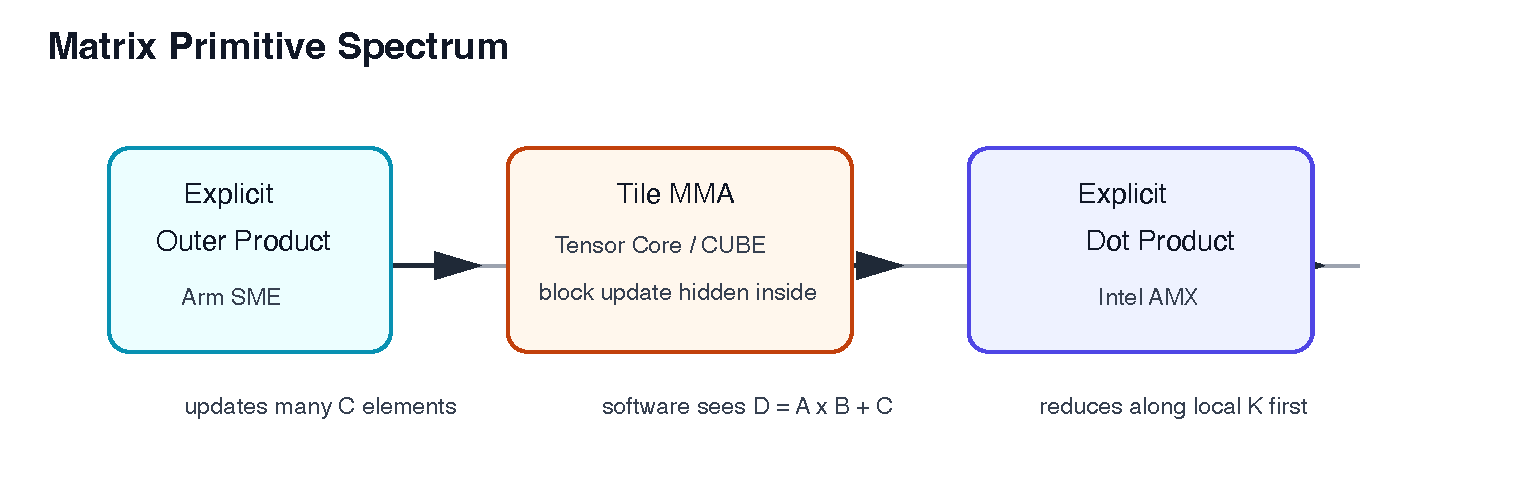
\includegraphics[width=0.9\textwidth]{figures/tile-mma-spectrum.pdf}
  \caption{公开矩阵原语的一个直观谱系：SME 在 ISA 层显式暴露 outer product，AMX 显式暴露 dot product，
  Tensor Core 与 CUBE 则把软件接口停在 tile MMA 层。}
  \label{fig:primitive-spectrum}
\end{figure}

\noindent\textbf{Algorithm 4.} SME-style outer-product tile update
\begin{code}
load ZA tile
for each k-step:
  a_vec = load vector from A
  b_vec = load vector from B
  ZA += outer_product(a_vec, b_vec)
store ZA tile
\end{code}

\noindent\textbf{Algorithm 5.} AMX-style dot-product tile update
\begin{code}
load dst tile
for each local K chunk:
  a_tile = load tile from A
  b_tile = load tile from B
  dst += dot_product_reduce(a_tile, b_tile)
store dst tile
\end{code}

\section{对 \outercube{} 的重构}

\subsection{公开规格中的基本设计点}

\outercube{} 文档把自身定义为 ``outer-product accumulation engine''，并给出以下核心
要点：8 个 bank，每个 bank 为 $8 \times 64$ MAC 阵列；支持 FP16/BF16/FP8/MXFP4/HiFP4；
所有格式统一累加到 32-bit FP32 accumulator；提供 \modea{} 和 \modeb{} 两种运行模式
\cite{outercube}.

在 \modea{} 中，8 个 bank 处理不同 K-group，inter-bank adder tree 将 8 个 bank 的部分和
归约到一个共享 accumulator 上；在 \modeb{} 中，8 个 bank 分别处理不同 M-block，bypass
inter-bank tree，每个 bank 都保有自己的 accumulator \cite{outercube}.

\subsection{\modea{} 与 \modeb{} 的局部归约深度}

如果按照文档中的微结构伪代码重写局部归约深度，可以得到：

\begin{itemize}
  \item \modea{}：
  \begin{itemize}
    \item FP16/BF16：每个 bank 每步处理 1 个乘积，8 bank inter-bank reduction 后再更新 ACC，
    故 $\ku = 8$。
    \item FP8：每个 MAC 先做 2-way local dot product，再经 8 bank reduction，故 $\ku = 16$。
    \item FP4：每个 MAC 先做 8-way local reduction，再经 8 bank reduction，故 $\ku = 64$。
  \end{itemize}
  \item \modeb{}：
  \begin{itemize}
    \item FP16/BF16：无 inter-bank reduction，故 $\ku = 1$。
    \item FP8：只有每 MAC 内的 2-way reduction，故 $\ku = 2$。
    \item FP4：只有每 MAC 内的 8-way reduction，故 $\ku = 8$。
  \end{itemize}
\end{itemize}

也就是说，\modea{} 并非 naive outer product；它已经是 ``块外积 + 局部小点积'' 的折中。
而 \modeb{} 在 FP16/FP8 下则退化到很小的 $\ku$，这正是其最根本的电路风险。

\begin{figure}[H]
  \centering
  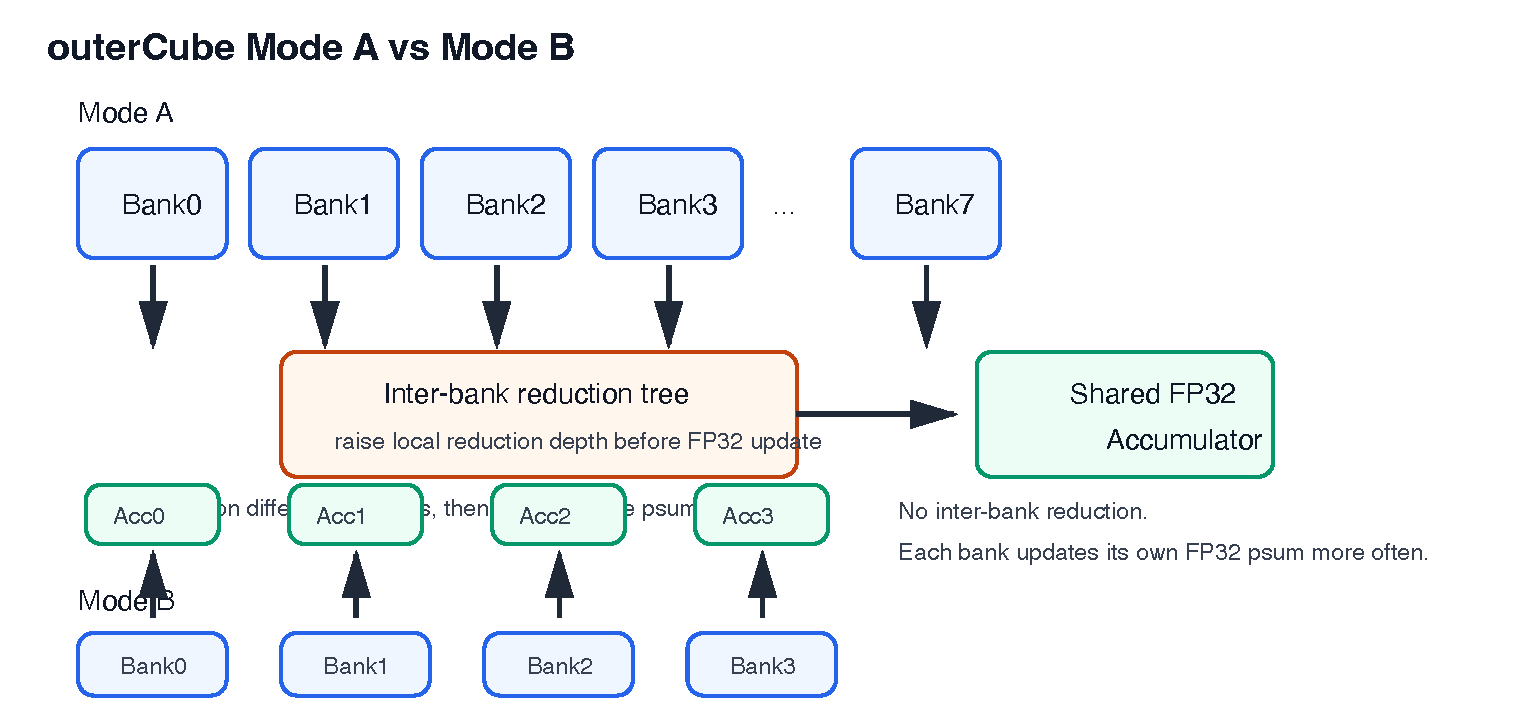
\includegraphics[width=0.92\textwidth]{figures/outercube-modes.pdf}
  \caption{\outercube{} 的两种模式示意。\modea{} 先做 inter-bank reduction，再更新共享 FP32 psum；
  \modeb{} 绕过 inter-bank reduction，由每个 bank 更频繁地更新自己的 FP32 psum。}
  \label{fig:outercube-modes}
\end{figure}

\noindent\textbf{Algorithm 6.} \modea{} simplified flow
\begin{code}
for each K-group:
  for bank in 0 .. 7:
    partial[bank] = local_mac_reduce(bank)
  merged = inter_bank_reduce(partial[0..7])
  shared_acc += merged
\end{code}

\noindent\textbf{Algorithm 7.} \modeb{} simplified flow
\begin{code}
for each K-group:
  for bank in 0 .. 7:
    partial = local_mac_reduce(bank)
    private_acc[bank] += partial
\end{code}

\subsection{FP32 更新频率的相对关系}

对同样的完整 K 归约长度，high-precision psum 更新次数与 $1/\ku$ 成正比。于是：

\begin{itemize}
  \item FP16：\modeb{} 的 FP32 更新频率是 \modea{} 的 8 倍。
  \item FP8：\modeb{} 的 FP32 更新频率是 \modea{} 的 8 倍。
  \item FP4：\modeb{} 的 FP32 更新频率仍是 \modea{} 的 8 倍。
\end{itemize}

这个 ``8 倍'' 很关键，因为它说明 \modeb{} 并不是只在 K 粒度上更细，它同时也把 floating-point
accumulation 的触发频率放大了 8 倍。

\section{\outercube{} 的主要优点}

\subsection{\modea{} 选择了合理的 dense GEMM 主数据流}

如果只看 dense low-precision GEMM，\modea{} 的总体方向是合理的。

首先，它保留了 block outer-product 的高复用特征。8 个 bank 同时覆盖不同 K-group，但共享
同一输出 tile 的空间位置；这使其对 $A$ 与 $B$ 的复用更像 systolic / tensor-core 类数据流，
而不是大量独立 dot-product lane 的松散集合。对大 K 场景，这种组织通常比分散内积更容易获得
高利用率 \cite{tpu,blis}.

其次，\modea{} 不是每个乘积直接落到 FP32 accumulator，而是通过 cell 内 reduction 和
inter-bank reduction 先把归约深度提升到 $\ku=8/16/64$。这是一个很重要的设计点：它说明
\outercube{} 的强项恰恰在于 \textbf{它没有把自己实现成纯粹的小粒度外积更新}。

\subsection{统一 FP32 psum 让软件语义简单}

从编程模型角度看，统一 FP32 accumulator 有明显优点。

\begin{itemize}
  \item 各种输入格式都落到统一输出格式，软件不需要为 FP16、FP8、MXFP4 分别管理不同 psum 类型。
  \item tile-level ISA 可直接把 K 循环折叠进 `CUBE.OPA`，减轻软件调度负担。
  \item 对功能正确性和模型移植而言，``所有格式统一累加到 FP32'' 是一个很强的语义契约。
\end{itemize}

这也是为什么许多现实系统在低精度乘法之后仍保留更高精度的 accumulation \cite{deepseekv3,abs}.

\subsection{双模式覆盖了不同工作负载的直觉需求}

从算法映射角度，\modea{} 和 \modeb{} 分别对应两种常见诉求：

\begin{itemize}
  \item 大 K、dense、batch 不太大时，希望沿 K 方向并行，提高吞吐，这对应 \modea{}。
  \item 小 K、M 很大时，希望减少 K-ceiling waste，这对应 \modeb{}。
\end{itemize}

因此，\outercube{} 不是随意地把 ``内积'' 和 ``外积'' 拼在一起；它确实试图把工作负载几何形状纳入
执行模式设计，这一点是成熟的。

\subsection{不使用 B broadcast MUX 简化了关键数据通路}

文档明确拒绝在 \modeb{} 上引入 B broadcast MUX，理由是 4 个 B 端口已经足以消除性能瓶颈，
因此 broadcast 带来的主要收益只剩功耗，而非吞吐 \cite{outercube}. 从 timing-closure 视角看，
去掉大广播 MUX 的确有好处：

\begin{itemize}
  \item 少了一个跨 bank 的共享数据分配网络。
  \item Mode A 和 Mode B 共用同一条 TRegFile B 数据路径，更利于实现复用。
  \item 关键路径可以更多集中在 local MAC 与 reduction tree，而不是 global fanout。
\end{itemize}

这说明 \outercube{} 在若干地方明显偏向 ``把控制和路由做简单''，这种取舍在大阵列设计里是合理的。

\section{\outercube{} 的主要问题}

\subsection{\modeb{} 是小 $\ku$ 外积，在 FP16/FP8 下电路代价偏高}

这是本文最核心的负面结论。对于 \modeb{}：

\begin{itemize}
  \item FP16/BF16 的 $\ku = 1$；
  \item FP8 的 $\ku = 2$；
  \item FP4 的 $\ku = 8$。
\end{itemize}

这意味着 \modeb{} 特别接近知乎文章批评的那类设计：每来很少几个乘积，就要把结果并入 FP32
语义 psum。对浮点电路而言，这会同时放大以下代价：

\begin{itemize}
  \item exponent compare 与 alignment 的触发频率；
  \item normalization 与 rounding 的触发频率；
  \item psum 寄存与回写活动；
  \item high-precision adder 的动态翻转次数；
  \item drain 前 psum RAM 的写活动。
\end{itemize}

如果说 \modea{} 已经通过局部 reduction 把外积做成了 ``不那么 naive''，那么 \modeb{} 恰恰又把设计拉回到
了 ``高频率更新高精度 psum'' 的方向。

\subsection{reduced-precision adder tree 的精度叙述过强}

\outercube{} 文档给出一张 ``intra-MAC adder tree internal width'' 表，并进一步声称
tree output widened to FP32 时可以通过 zero-padding 实现 ``no precision loss'' \cite{outercube}.

这个表述在浮点电路语境下问题很大。原因不在于缩窄 adder tree 本身不可行，而在于：

\begin{itemize}
  \item 浮点加法误差不仅取决于 mantissa 位数，还取决于 exponent alignment。
  \item 多个操作数相加时需要 guard / round / sticky bits 以支持正确舍入。
  \item cancellation 可能让需要保留的有效位向高位与低位两侧同时扩展。
  \item ``mantissa 加 $\log_2 N$'' 更像定点求和的上界直觉，而不是 IEEE 浮点加法的完整精度模型。
\end{itemize}

Lutz 等人的 FP8-DOT4 设计恰恰说明，哪怕只是 4-way FP8 dot product with FP32 accumulation，
真正认真做的 SoP datapath 也会扩展到 69-bit adder 和 94-bit adder 量级 \cite{lutz2024}。
DeepSeek-V3 则进一步说明，现实 Hopper Tensor Core 在 FP8 GEMM 上因为只保留约 14 bit
accumulation precision，已经会对训练精度造成明显影响 \cite{deepseekv3}. 在这种背景下，
\outercube{} 的 ``缩窄 tree 仍无精度损失'' 若没有更严格的块浮点、exact fixed-point 或
受限舍入规则支持，按字面很难成立。

\subsection{统一 FP32 accumulator 虽然稳，但可能明显过度配置}

统一 FP32 accumulator 的软件语义很优雅，但从电路角度它也意味着明显 over-provisioning。

\begin{itemize}
  \item 对 FP4/MXFP4 这类格式，统一 FP32 psum 可能远宽于某些推理场景的必要精度。
  \item A2Q 已经表明 accumulator bit-width 是低精度硬件的重要优化自由度 \cite{a2q}。
  \item DGA 等工作则说明通过分组和两级 accumulation，可以在保持精度的同时缩减局部 accumulator 压力
  \cite{dga}.
\end{itemize}

因此，统一 FP32 的问题不在于 ``太保守''，而在于它把很多本可在局部层面做的数值优化都推迟到了
最贵的那一级。

\subsection{\modeb{} 的 drain 代价与其目标场景天然冲突}

\modeb{} 的另一个问题是 drain。文档明确写到：

\begin{itemize}
  \item \modea{} drain：2 KB，8 cycles。
  \item \modeb{} drain：16 KB，32 cycles。
\end{itemize}

注意 \modeb{} 的目标正是 ``small K, large M'' 场景。可一旦 K 变小，compute 时间缩短，而 16 KB
FP32 drain 却不会同比缩短。文档自己也给出例子说明 \modeb{} 在小 K 下容易 drain-limited
\cite{outercube}. 这说明 \modeb{} 虽然在算法上消除了 K-waste，但在电路上引入了更大的 psum
和 writeback 开销，二者未必对等。

\subsection{不做 B broadcast 虽然利于实现，但会放大数据流功耗}

文档强调 ``broadcast 性能收益为 0\%''，因此不引入 B broadcast MUX \cite{outercube}. 从吞吐看，
这没错；但从电路能耗看，问题并没有消失，而是被转移到了 TRegFile：

\begin{itemize}
  \item 8 个 bank 在 \modeb{} 中读取相同 B 数据，但依赖独立读取而非共享广播。
  \item 这减少了共享分发逻辑，却放大了 TRegFile 端口活动和 bank 读翻转。
  \item 根据 Eyeriss 等经验，数据移动代价常常比乘法本身更关键 \cite{eyeriss}.
\end{itemize}

因此，``不做 broadcast'' 是一个 timing 与实现复杂度上偏保守、在 energy 上偏激进的选择。
如果目标是低功耗矩阵单元，而非只追求路由简单，这一点需要重新权衡。

\subsection{accumulator 放置的语义不够清晰}

规格前半部分说 ``each physical MAC unit contains ... an FP32 accumulator''，
后面又说 \modea{} 是 8 bank 先 reduction 再进共享 accumulator \cite{outercube}. 这两种说法
对应两种完全不同的物理实现：

\begin{itemize}
  \item 若每 MAC 近端都有 FP32 accumulator，则局部状态量巨大，但 inter-bank reduction 可以在
  更高一级做。
  \item 若每个输出元素只在 bank 或全局级别持有一个 FP32 accumulator，则 state 更集中，但
  reduction tree 与 psum write path 会更重。
\end{itemize}

对于架构文档，这个歧义看似是表述问题；但对微架构评估，它直接决定面积、布线、时序与功耗的判断。

\section{与其它设计点的对比}

表 \ref{tab:compare} 总结了几类相关设计点。这里不讨论 ISA 是否暴露 dot-product 或 MMA，
而只关心电路层最核心的局部归约粒度、psum 更新频率和主要风险。

\begin{table}[H]
  \centering
  \caption{几类矩阵乘设计点与公开矩阵原语的电路级对比}
  \label{tab:compare}
  \begin{tabularx}{\textwidth}{>{\raggedright\arraybackslash}p{2.5cm} >{\raggedright\arraybackslash}p{2.3cm} >{\raggedright\arraybackslash}p{1.45cm} >{\raggedright\arraybackslash}X >{\raggedright\arraybackslash}X}
    \toprule
    设计点 & 主数据流 & 典型 $\ku$ & 主要优点 & 主要风险 \\
    \midrule
    naive outer update & 外积 & 1 & 结构简单，控制直观 & FP psum 更新过频，数值与功耗都差 \\
    Arm SME & 显式外积 & ISA 未显式固定 & 语义直接，ZA tile 与 outer-product accumulate 一一对应 & 电路质量仍取决于底层实现的局部归约与 psum 组织 \\
    Intel AMX & 显式 dot product & ISA 未显式固定 & 点积语义清晰，局部 K 归约自然暴露 & SoP 对齐、宽 datapath 与 accumulator 代价集中在点积单元 \\
    NVIDIA Tensor Core & tile MMA / 块外积 & 实现相关 & tile 级 MMA 接口紧凑，适合高复用 block update & 软件接口不直接暴露局部归约深度，数值代价依赖底层 accumulation 设计 \\
    DaVinci CUBE & tile MMA / systolic 更新 & 实现相关 & 与 systolic 阵列配合自然，tile GEMM 吞吐高 & 公开资料较少，局部 primitive 与数值路径不够透明 \\
    \outercube{} \modea{} & 块外积 + 局部归约 & 8 / 16 / 64 & dense GEMM 友好，复用高，FP32 更新频率可接受 & 仍需认真处理 floating-point tree 精度 \\
    \outercube{} \modeb{} & 小 $\ku$ 外积 & 1 / 2 / 8 & 小 K 时减少 K-ceiling waste & FP32 更新频率高，drain 重，TRegFile 读流量大 \\
    FP8-DOT4 / DOT8 单元 & 小内积 & 4 / 8 & 显著减少 high-precision accumulation 频率 & SoP 对齐与宽 datapath 代价高 \\
    exact dot product & 大内积 & 极大 & 数值最强，可复现性好 & accumulator 极宽，面积和时序都重 \\
    \bottomrule
  \end{tabularx}
\end{table}

这张表的重点不是证明 ``内积优于外积''，而是说明：\textbf{真正好的设计通常既不是纯外积，也不是纯内积，
而是 block outer-product 加上适中的 local dot-product depth。}

\section{架构决策框架}

到这里，论文的核心结论已经可以从“评审一个设计”上升到“如何选择一类设计”。综合来看，
\outercube{} 的价值和问题都说明了一点：真正需要做决策的，并不是抽象地站队“内积”或“外积”，
而是决定 \textbf{主数据流、局部归约深度和 accumulator 介入频率} 这三件事情如何组合。

因此，\outercube{} 的核心价值不应被概括为
``outer-product accumulation engine'' 这一标签本身，而应被理解为：

\begin{quote}
  \outercube{} 的核心并不在于单纯采用 outer-product accumulation，而在于通过
  block outer-product dataflow 维持 dense GEMM 吞吐，并通过局部 reduction depth
  的选择在 arithmetic cost、numerical robustness 和 psum bandwidth 之间折中。
\end{quote}

在这一框架下，\outercube{} 的优点、风险与适用边界可以更清晰地表述为：

\begin{enumerate}
  \item \textbf{架构优点}：
  \modea{} 对 dense GEMM 合理；tile-level ISA 简化软件；统一 accumulator 简化语义。
  \item \textbf{电路风险}：
  \modeb{} 的局部归约深度过小；reduced-precision tree 需要更严格的数值证明；统一 FP32
  accumulator 与大 drain 让小 K 路线代价偏高。
  \item \textbf{边界条件}：
  如果目标是大 K dense GEMM，\modea{} 很有价值；如果目标是 FP8 训练友好或更广义的 low-bit
  GEMM，\modeb{} 当前形态不够稳健。
\end{enumerate}

\subsection{如何在 inner 与 outer 之间做选择}

对真正做架构决策的人而言，最有用的问题通常不是“某个单元属于哪一派”，而是下面三个问题：

\begin{enumerate}
  \item \textbf{吞吐与复用的主矛盾是什么？}
  如果主要矛盾是 dense GEMM 中输入 tile 的高复用和规则数据流，那么 outer-product 或
  block outer-product 往往更自然；如果主要矛盾是沿局部 K 维做紧凑归约、并把 primitive
  直接暴露为 dot-product 或 small SoP，那么 inner-product primitive 更自然。
  \item \textbf{能接受多高的 high-precision psum 更新频率？}
  如果数值、能耗或时序预算不允许 accumulator 在 product 级频繁介入，那么就必须提高 \ku{}，
  用 local dot、grouped reduction 或 tree reduction 把更新频率降下来。
  \item \textbf{软件接口需要暴露什么层级的抽象？}
  若希望软件直接编排 outer-product tile update，SME 一类显式 outer-product primitive
  更合适；若希望软件直接获得 dot-product 语义，AMX 一类接口更直观；若希望把实现自由度留给
  硬件，则 tile MMA 接口通常是更稳妥的折中。
\end{enumerate}

\subsection{决策导图}

\begin{table}[H]
  \centering
  \caption{面向架构决策的 inner / outer 选择建议}
  \label{tab:decision}
  \begin{tabularx}{\textwidth}{>{\raggedright\arraybackslash}p{3.0cm} >{\raggedright\arraybackslash}p{3.3cm} >{\raggedright\arraybackslash}X}
    \toprule
    场景或约束 & 更合适的方向 & 主要理由 \\
    \midrule
    大 K、dense GEMM、规则 tile & block outer-product + local reduction & 输入复用高，数据流规则；但必须避免 $\ku=1$ 的 product 级高频 psum 更新 \\
    小 K、需要明确局部 K 归约语义 & inner-product primitive / grouped dot product & accumulator 介入次数更少，数值路径更可控，软件语义也更直接 \\
    既要高吞吐又要保留实现自由度 & tile MMA & 软件看到统一的 $D=A\times B+C$，硬件可自行选择外积数据流或局部分组归约 \\
    FP16/BF16/FP8，精度风险敏感 & 避免纯串行 outer accumulation & 应优先提高 \ku{}，把 sequential accumulation 改成 grouped 或 tree-style accumulation \\
    极度强调结果可解释性或高精度 contract & dot-product / exact-style accumulation & 舍入点更少，误差边界更容易分析，但面积和时序代价更高 \\
    \bottomrule
  \end{tabularx}
\end{table}

\subsection{本文给出的最终判断}

基于全文分析，本文给出如下判断：

\begin{itemize}
  \item 不存在脱离工作负载、数值 contract 和实现预算的“内积必优”或“外积必优”。
  \item 对现代低精度 dense GEMM，最稳妥的方向通常不是纯 inner，也不是纯 outer，而是
  \textbf{block outer-product dataflow + 适中的 local dot-product depth}。
  \item 对 FP16/BF16/FP8 而言，真正应避免的是 \textbf{\ku{} 过小}，因为这会让 unified accumulator
  在 product 级反复参与对齐和舍入，既伤精度也伤能效。
  \item 因而，如果今天必须在“纯内积”和“纯外积”之间二选一，本文更反对的是
  \textbf{纯外积串行累加}；如果允许现实工程中的混合方案，本文更支持的是
  \textbf{外积主数据流配局部 dot/reduction}。
\end{itemize}

\section{对下一版设计的建议}

\subsection{保留 \modea{}，重写 \modeb{}}

\modea{} 是 \outercube{} 最像成熟产品的部分，应当保留。真正需要重写的是 \modeb{}。
更合理的方向不是继续坚持 ``每步 K 更细''，而是：

\begin{itemize}
  \item 为 \modeb{} 增加明确的 chunk accumulation 或 grouped accumulation。
  \item 把 $\ku$ 至少从 1/2/8 提高到 4/8/16 甚至更高。
  \item 用局部 SoP buffer 或 partial accumulator 暂存结果，降低 FP32 更新频率。
\end{itemize}

\subsection{把数值格式当成一等设计对象}

如果 \outercube{} 想在 FP8 与 MXFP4 上进一步前进，单靠统一 FP32 accumulator 不够。更值得引入的是：

\begin{itemize}
  \item microscaling / block scaling，与 K 维局部分组对齐 \cite{mx};
  \item group accumulation / dynamic group accumulation \cite{dga};
  \item 对敏感路径显式支持 higher-precision promotion，而不是把所有路径都推到 FP32 \cite{deepseekv3}.
\end{itemize}

\subsection{重新表述 reduced-precision tree}

若要保留 reduced-precision tree 作为卖点，论文必须给出更严谨的表述：

\begin{itemize}
  \item 若它是近似求和，应明确误差模型与适用范围；
  \item 若它是 exact 或 no-loss，需要给出对 exponent alignment、guard/sticky 与 rounding 的完整证明；
  \item 若它实际是块浮点或共享指数形式，则必须把数据格式定义写成规范，而不是只给 mantissa 位宽表。
\end{itemize}

\subsection{重新审视 B broadcast 的能效取舍}

不做 broadcast 可以继续作为 baseline，但建议至少研究两个版本：

\begin{itemize}
  \item 低复杂度无 broadcast 版本：更容易实现；
  \item 能效优化 broadcast 版本：减少 TRegFile 重复读取。
\end{itemize}

在 large-M small-K 场景下，哪种更优，不应只用吞吐判断，还应看 SRAM read energy 与 total joules/op。

\section{结论}

\outercube{} 不是一个简单的“外积机”，而是一个把外积数据流、局部 dot/reduction 与 unified FP32
accumulation 混合在一起的矩阵单元。本文的分析表明，真正决定其好坏的，并不是它在标签上更像 inner
还是 outer，而是局部归约深度 \ku{} 是否足够大、high-precision psum 是否被过于频繁地触发，以及
数值路径是否被清晰而严格地定义。

对本文关心的架构决策而言，可以把最终结论压缩为三句话。第一，\modea{} 代表了一条合理的工程方向：
用 block outer-product dataflow 获取复用和吞吐，再用局部 reduction 控制 FP32 accumulator 的介入频率。
第二，\modeb{} 揭示了一个明确的风险边界：当 \ku{} 过小，设计就会从“高复用的外积数据流”退化为“product 级
高频更新高精度 psum”的顺序累加机。第三，现代低精度矩阵乘单元最稳妥的答案通常不是纯 inner 或纯 outer，
而是二者的受控组合。

因此，如果目标是为后续架构设计提供可操作的判断标准，本文的建议是：
\begin{itemize}
  \item 当工作负载以大 K dense GEMM 为主时，优先采用 block outer-product dataflow，但必须显式设计
  local dot/reduction、group accumulation 或 tree accumulation，避免 $\ku=1$。
  \item 当工作负载更偏小 K、对局部 K 归约语义更敏感、或对数值行为需要更强可解释性时，优先考虑
  inner-product primitive 或 grouped dot-product primitive。
  \item 当 ISA 需要保持中性、又希望给硬件保留足够实现自由度时，tile MMA 往往是更现实的接口层折中。
\end{itemize}

换句话说，真正该避免的不是“外积”本身，而是 \textbf{缺乏局部归约深度的纯串行外积累加}；
真正值得优先考虑的，也不是抽象意义上的“内积”或“外积”，而是是否能够把
\textbf{数据复用、局部归约和高精度 psum 更新频率} 这三件事同时处理好。

\begin{thebibliography}{99}

\bibitem{outercube}
Heng Liao.
\newblock \emph{outerCube Design}.
\newblock GitHub repository document, 2026.
\newblock \url{https://github.com/hengliao1972/pyCircuit/tree/main/designs/outerCube}

\bibitem{blis}
Tyler M. Smith, Robert A. van de Geijn, M. Smelyanskiy, Jeff R. Hammond, and Field G. Van Zee.
\newblock Analytical Modeling Is Enough for High-Performance BLIS.
\newblock \emph{ACM Transactions on Mathematical Software}, 2018.
\newblock \url{https://www.cs.utexas.edu/~flame/pubs/flawn74.pdf}

\bibitem{tpu}
Norman P. Jouppi et al.
\newblock In-Datacenter Performance Analysis of a Tensor Processing Unit.
\newblock In \emph{ISCA}, 2017.
\newblock \url{https://arxiv.org/abs/1704.04760}

\bibitem{eyeriss}
Yu-Hsin Chen, Tushar Krishna, Joel S. Emer, and Vivienne Sze.
\newblock Eyeriss: An Energy-Efficient Reconfigurable Accelerator for Deep Convolutional Neural Networks.
\newblock \emph{IEEE Journal of Solid-State Circuits}, 2017.
\newblock \url{https://people.csail.mit.edu/emer/media/papers/2016.06.isca.eyeriss_architecture.pdf}

\bibitem{abs}
Charbel Sakr et al.
\newblock Accumulation Bit-Width Scaling For Ultra-Low Precision Training Of Deep Networks.
\newblock In \emph{ICLR}, 2019.
\newblock \url{https://arxiv.org/abs/1901.06588}

\bibitem{a2q}
Ian Colbert, Alessandro Pappalardo, and Jakoba Petri-Koenig.
\newblock A2Q: Accumulator-Aware Quantization with Guaranteed Overflow Avoidance.
\newblock In \emph{ICCV}, 2023.
\newblock \url{https://openaccess.thecvf.com/content/ICCV2023/papers/Colbert_A2Q_Accumulator-Aware_Quantization_with_Guaranteed_Overflow_Avoidance_ICCV_2023_paper.pdf}

\bibitem{dga}
Yixiong Yang et al.
\newblock Toward Low-Bit Neural Network Training Accelerator by Dynamic Group Accumulation.
\newblock ASP-DAC tutorial material, 2022.
\newblock \url{https://aspdac2022.github.io/taoka/pdf/6C-2.pdf}

\bibitem{lutz2024}
David Raymond Lutz, Anisha Saini, Mairin Kroes, Thomas Elmer, and Harsha Valsaraju.
\newblock Fused FP8 4-Way Dot Product With Scaling and FP32 Accumulation.
\newblock In \emph{ARITH}, 2024.
\newblock \url{https://www.ac.uma.es/arith2024/papers/Fused%20FP8%204-Way%20Dot%20Product%20with%20Scaling%20and%20FP32%20Accumulation.pdf}

\bibitem{exactdot}
Jack Koenig.
\newblock A Hardware Accelerator for Computing an Exact Dot Product.
\newblock UC Berkeley Technical Report UCB/EECS-2018-51, 2018.
\newblock \url{https://www2.eecs.berkeley.edu/Pubs/TechRpts/2018/EECS-2018-51.pdf}

\bibitem{higham}
Nicholas J. Higham.
\newblock The Accuracy of Floating Point Summation.
\newblock \emph{SIAM Journal on Scientific Computing}, 14(4):783--799, 1993.
\newblock \url{https://nhigham.com/wp-content/uploads/2023/10/high93s.pdf}

\bibitem{smeintro}
Arm.
\newblock Arm Scalable Matrix Extension Introduction.
\newblock Arm developer documentation.
\newblock \url{https://developer.arm.com/documentation/109246/latest/}

\bibitem{smeinst}
Arm.
\newblock FMOPA, BFMOPA, and related SME instructions.
\newblock Arm Architecture Reference Manual for A-profile architecture supplement.
\newblock \url{https://developer.arm.com/documentation/ddi0616/latest/}

\bibitem{amxbf16}
Intel.
\newblock \_tile\_dpbf16ps: Compute dot-product of BF16 pairs in tiles.
\newblock Intel oneAPI DPC++/C++ Compiler Developer Guide and Reference.
\newblock \url{https://www.intel.com/content/www/us/en/docs/dpcpp-cpp-compiler/developer-guide-reference/current/tile-dpbf16ps.html}

\bibitem{amxsample}
Intel.
\newblock Advanced Matrix Extensions Intrinsics Functions.
\newblock Intel developer article and code sample.
\newblock \url{https://www.intel.com/content/www/us/en/developer/articles/code-sample/advanced-matrix-extensions-intrinsics-functions.html}

\bibitem{ptxisa}
NVIDIA.
\newblock Parallel Thread Execution ISA: Matrix multiply-accumulate instructions.
\newblock NVIDIA documentation.
\newblock \url{https://docs.nvidia.com/cuda/parallel-thread-execution/}

\bibitem{cutlass}
NVIDIA.
\newblock CUTLASS GEMM API.
\newblock NVIDIA documentation.
\newblock \url{https://docs.nvidia.com/cutlass/media/docs/cpp/gemm_api.html}

\bibitem{ascendmmad}
Huawei.
\newblock Mmad matrix multiply-accumulate API.
\newblock Ascend C API documentation.
\newblock \url{https://www.hiascend.com/document/detail/zh/CANNCommunityEdition/800alpha003/apiref/ascendcopapi/atlasascendc_api_07_0249.html}

\bibitem{davinci}
Marc Salvad\'o, Josep L. Briz, and Miquel Moret\'o.
\newblock Exploring the DaVinci Machine Learning Accelerator Architecture via Software-Hardware Simulation.
\newblock In \emph{International Conference on High Performance Computing \& Simulation Workshops}, 2021.
\newblock \url{https://webdocs.cs.ualberta.ca/~csalvado/publication/2021-pooling-acceleration-in-davinci/pooling-acceleration-in-davinci.pdf}

\bibitem{deepseekv3}
DeepSeek-AI.
\newblock DeepSeek-V3 Technical Report.
\newblock arXiv:2412.19437, 2024.
\newblock \url{https://arxiv.org/abs/2412.19437}

\bibitem{mx}
Bita Darvish Rouhani et al.
\newblock Microscaling Data Formats for Deep Learning.
\newblock arXiv:2310.10537, 2023.
\newblock \url{https://doi.org/10.48550/arXiv.2310.10537}

\end{thebibliography}

\end{document}
